\documentclass[12pt]{article}

%packages
\usepackage{fancyhdr}
\usepackage[margin=1in]{geometry}
\usepackage[utf8]{inputenc}
\usepackage{listings}
\usepackage{booktabs}
\usepackage{enumitem}
\usepackage{pdfpages}
\usepackage{graphicx}
\usepackage{listings}
\usepackage{xcolor}
\usepackage{subcaption}
\usepackage{float}
\usepackage{amsmath}

%fancyheadr fix
\setlength{\headheight}{15pt}

%commands to lslistings
\lstset{
    basicstyle=\ttfamily\small,
    breaklines=true,     
    breakatwhitespace=true,
    frame=single,
    numbers=left,
    numberstyle=\tiny,
    columns=fullflexible,
    keepspaces=true
}


%title info
\newcommand{\doctitle}{STA 5635 HW 6}
\newcommand{\name}{Palmer Swanson}
\newcommand{\docdate}{\today}

%document
\begin{document}

\begin{center}
    {\Large \doctitle}\\[6pt]
    {\name}\\[3pt]
    {\docdate}
\end{center}
\vspace{12pt}

\section*{Problem 1}

\begin{enumerate}[label=(1\alph*), ref=1\alph*]
    \item Two random forest classifiers.  One with 22 features, the other with 500.  Table in figure 
    \ref{tab:table_part_a}
    \begin{table}[htbp]
        \centering
        \input{../output/train_test_errors_a.tex}
        \caption{Train and Test Misclassification Errors, part a}
        \label{tab:table_part_a}
    \end{table}
    \item Compute feature importances using mean decrease in impurity and the permutation feature importances.
    \begin{figure}[htbp] 
        \centering 
        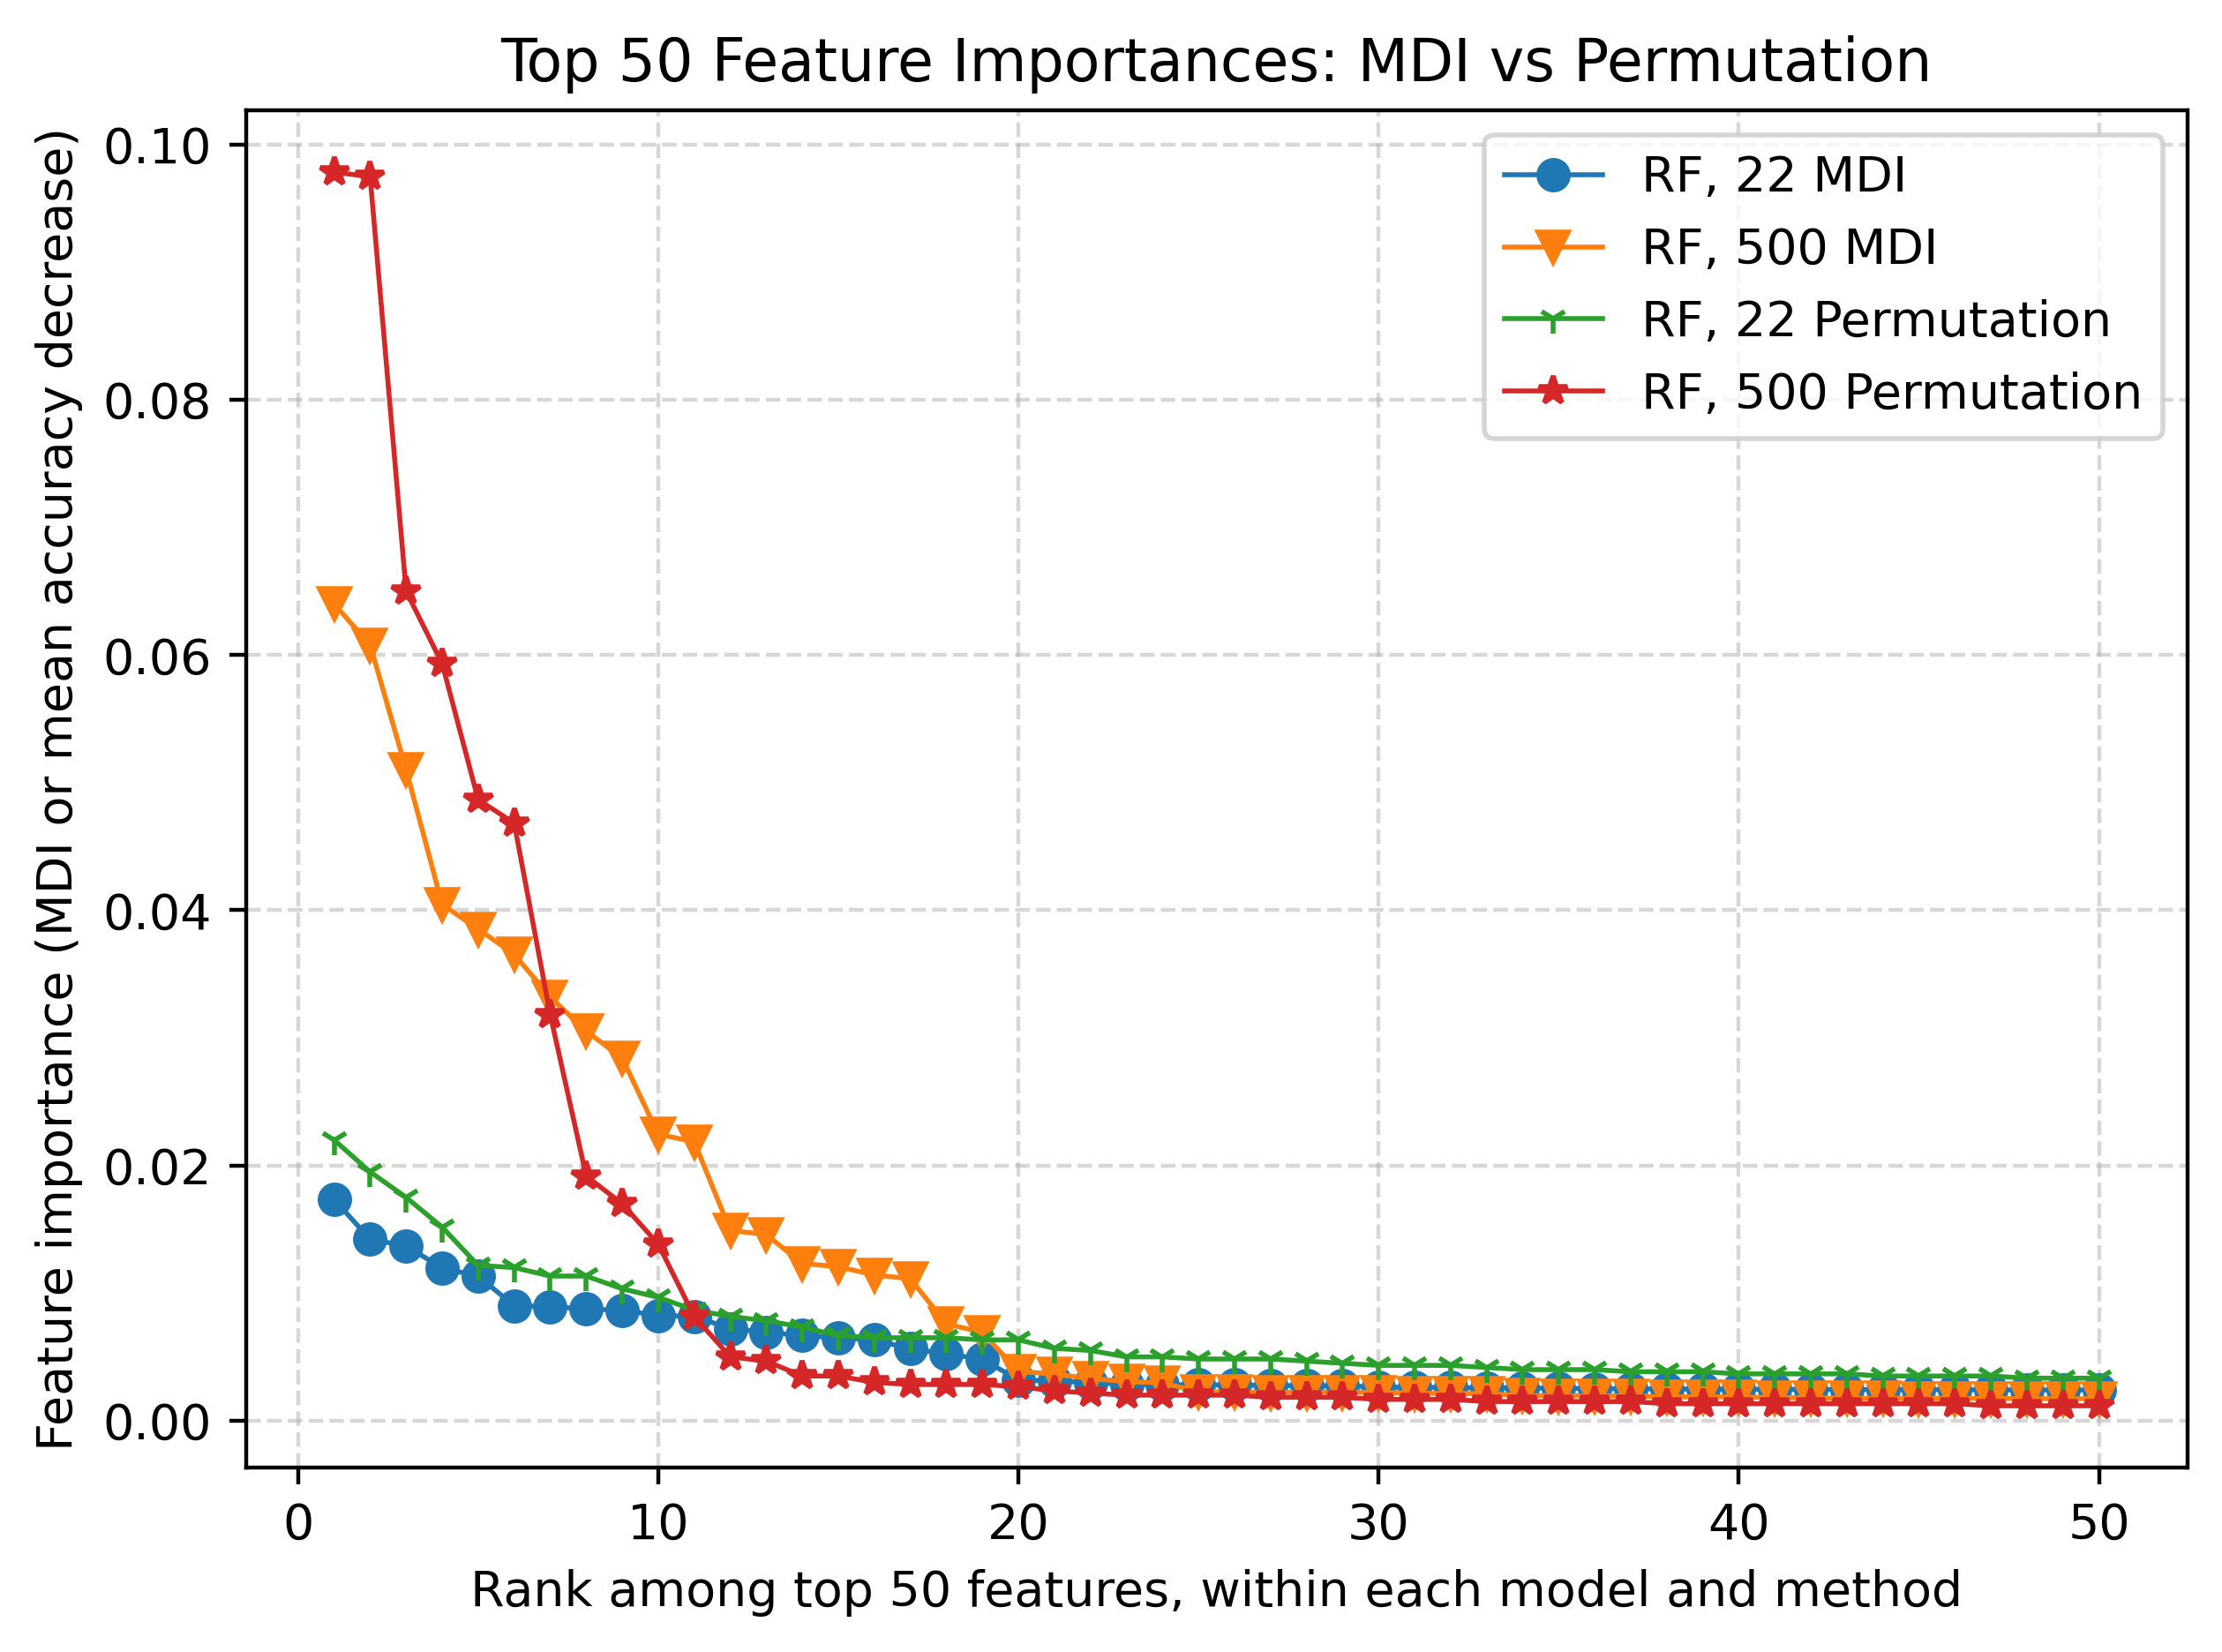
\includegraphics[width=0.7\linewidth]{../figures/feature_importances.png} 
        \caption{Feature Importances for the two RF, computed via MDI and via Permutations, part b.} 
    \label{fig:feature_importance} 
    \end{figure}
    \item Selecting \(k \in\{10, 20, 30, 40\}\) most important features by the two methods on the two classifiers, 
    train RF classifier.  The test and train errors are reported in table \ref{tab:table_part_c}.  
    \begin{table}[htbp]
        \centering
        \input{../output/train_test_errors_c.tex}
        \caption{Training and test misclassification errors for the fitted models, part c.}
        \label{tab:table_part_c}
    \end{table}
    \item For \(k \in\{10, 20, 30, 40\}\), two plots, one of each depth \(d\).  
    \(d=4\) is figure \ref{fig:test_error_d4}, \(d=5\)
    found in figure \ref{fig:test_error_d5}.  
    \begin{figure}[htbp] 
        \centering 
        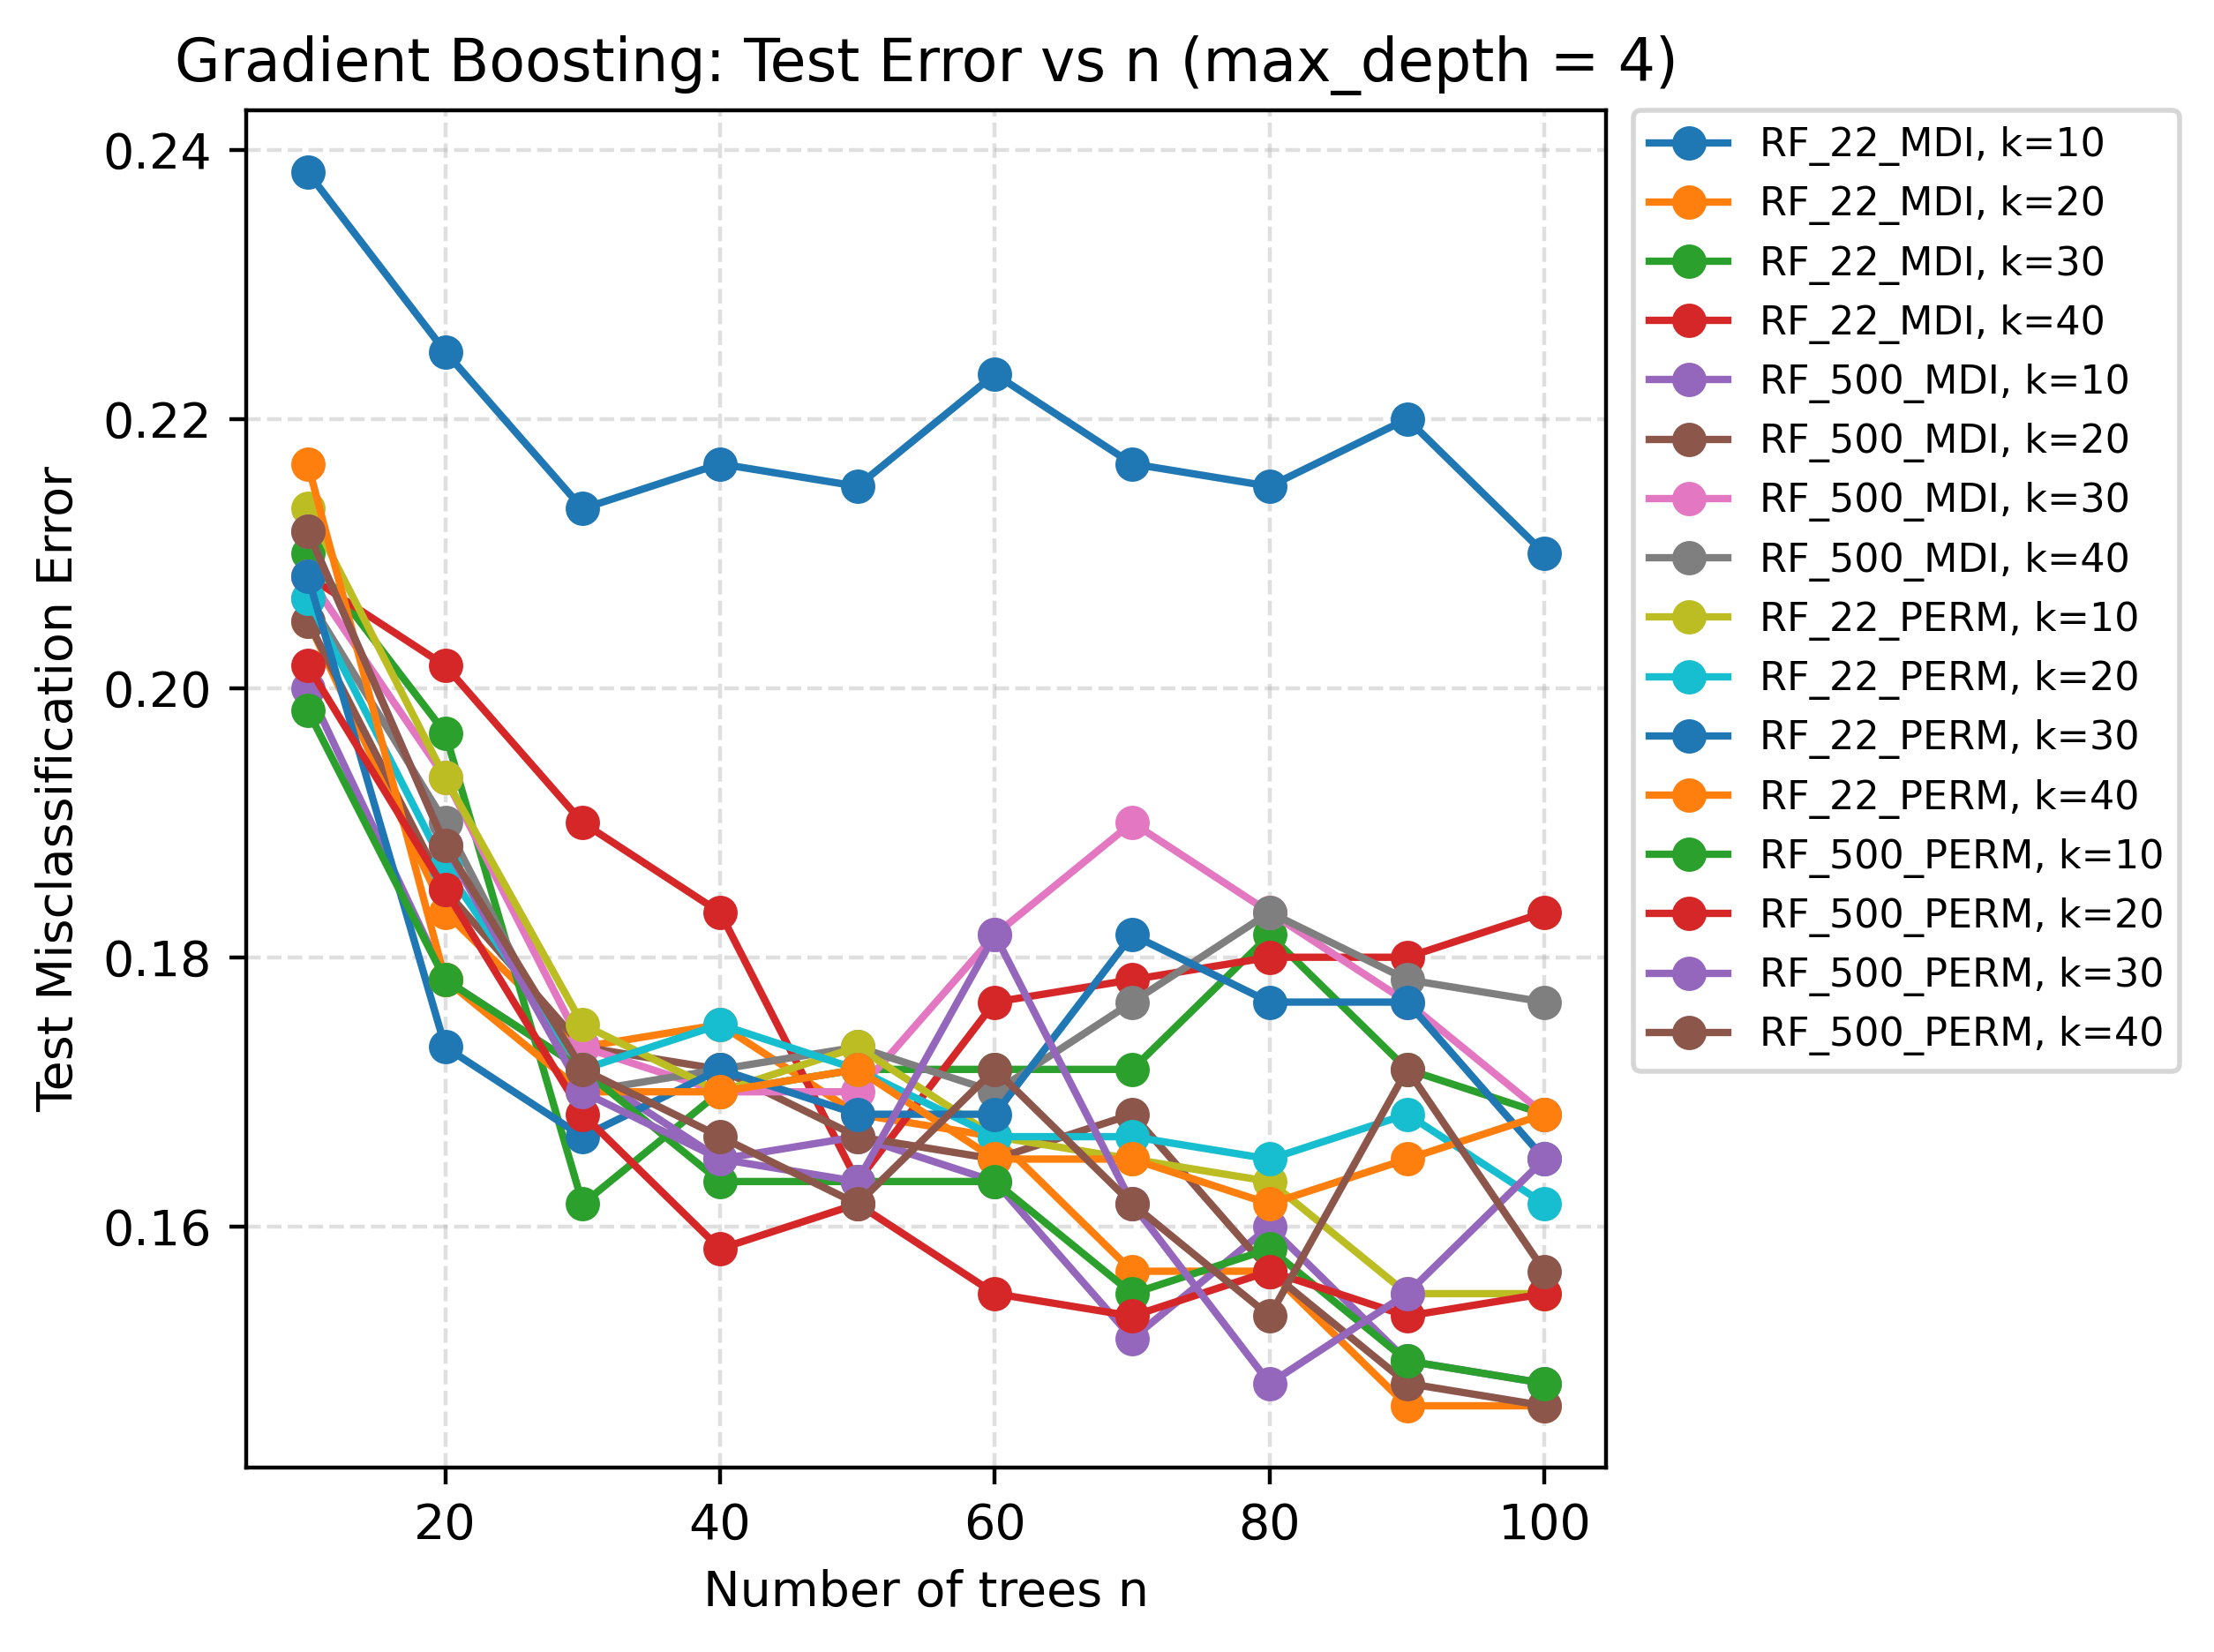
\includegraphics[width=0.7\linewidth]{../figures/gb_test_error_depth_4.png} 
        \caption{Test Errors vs. \(n\) for the 16 classifiers.  d=4} 
    \label{fig:test_error_d4} 
    \end{figure}
    \begin{figure}[htbp] 
        \centering 
        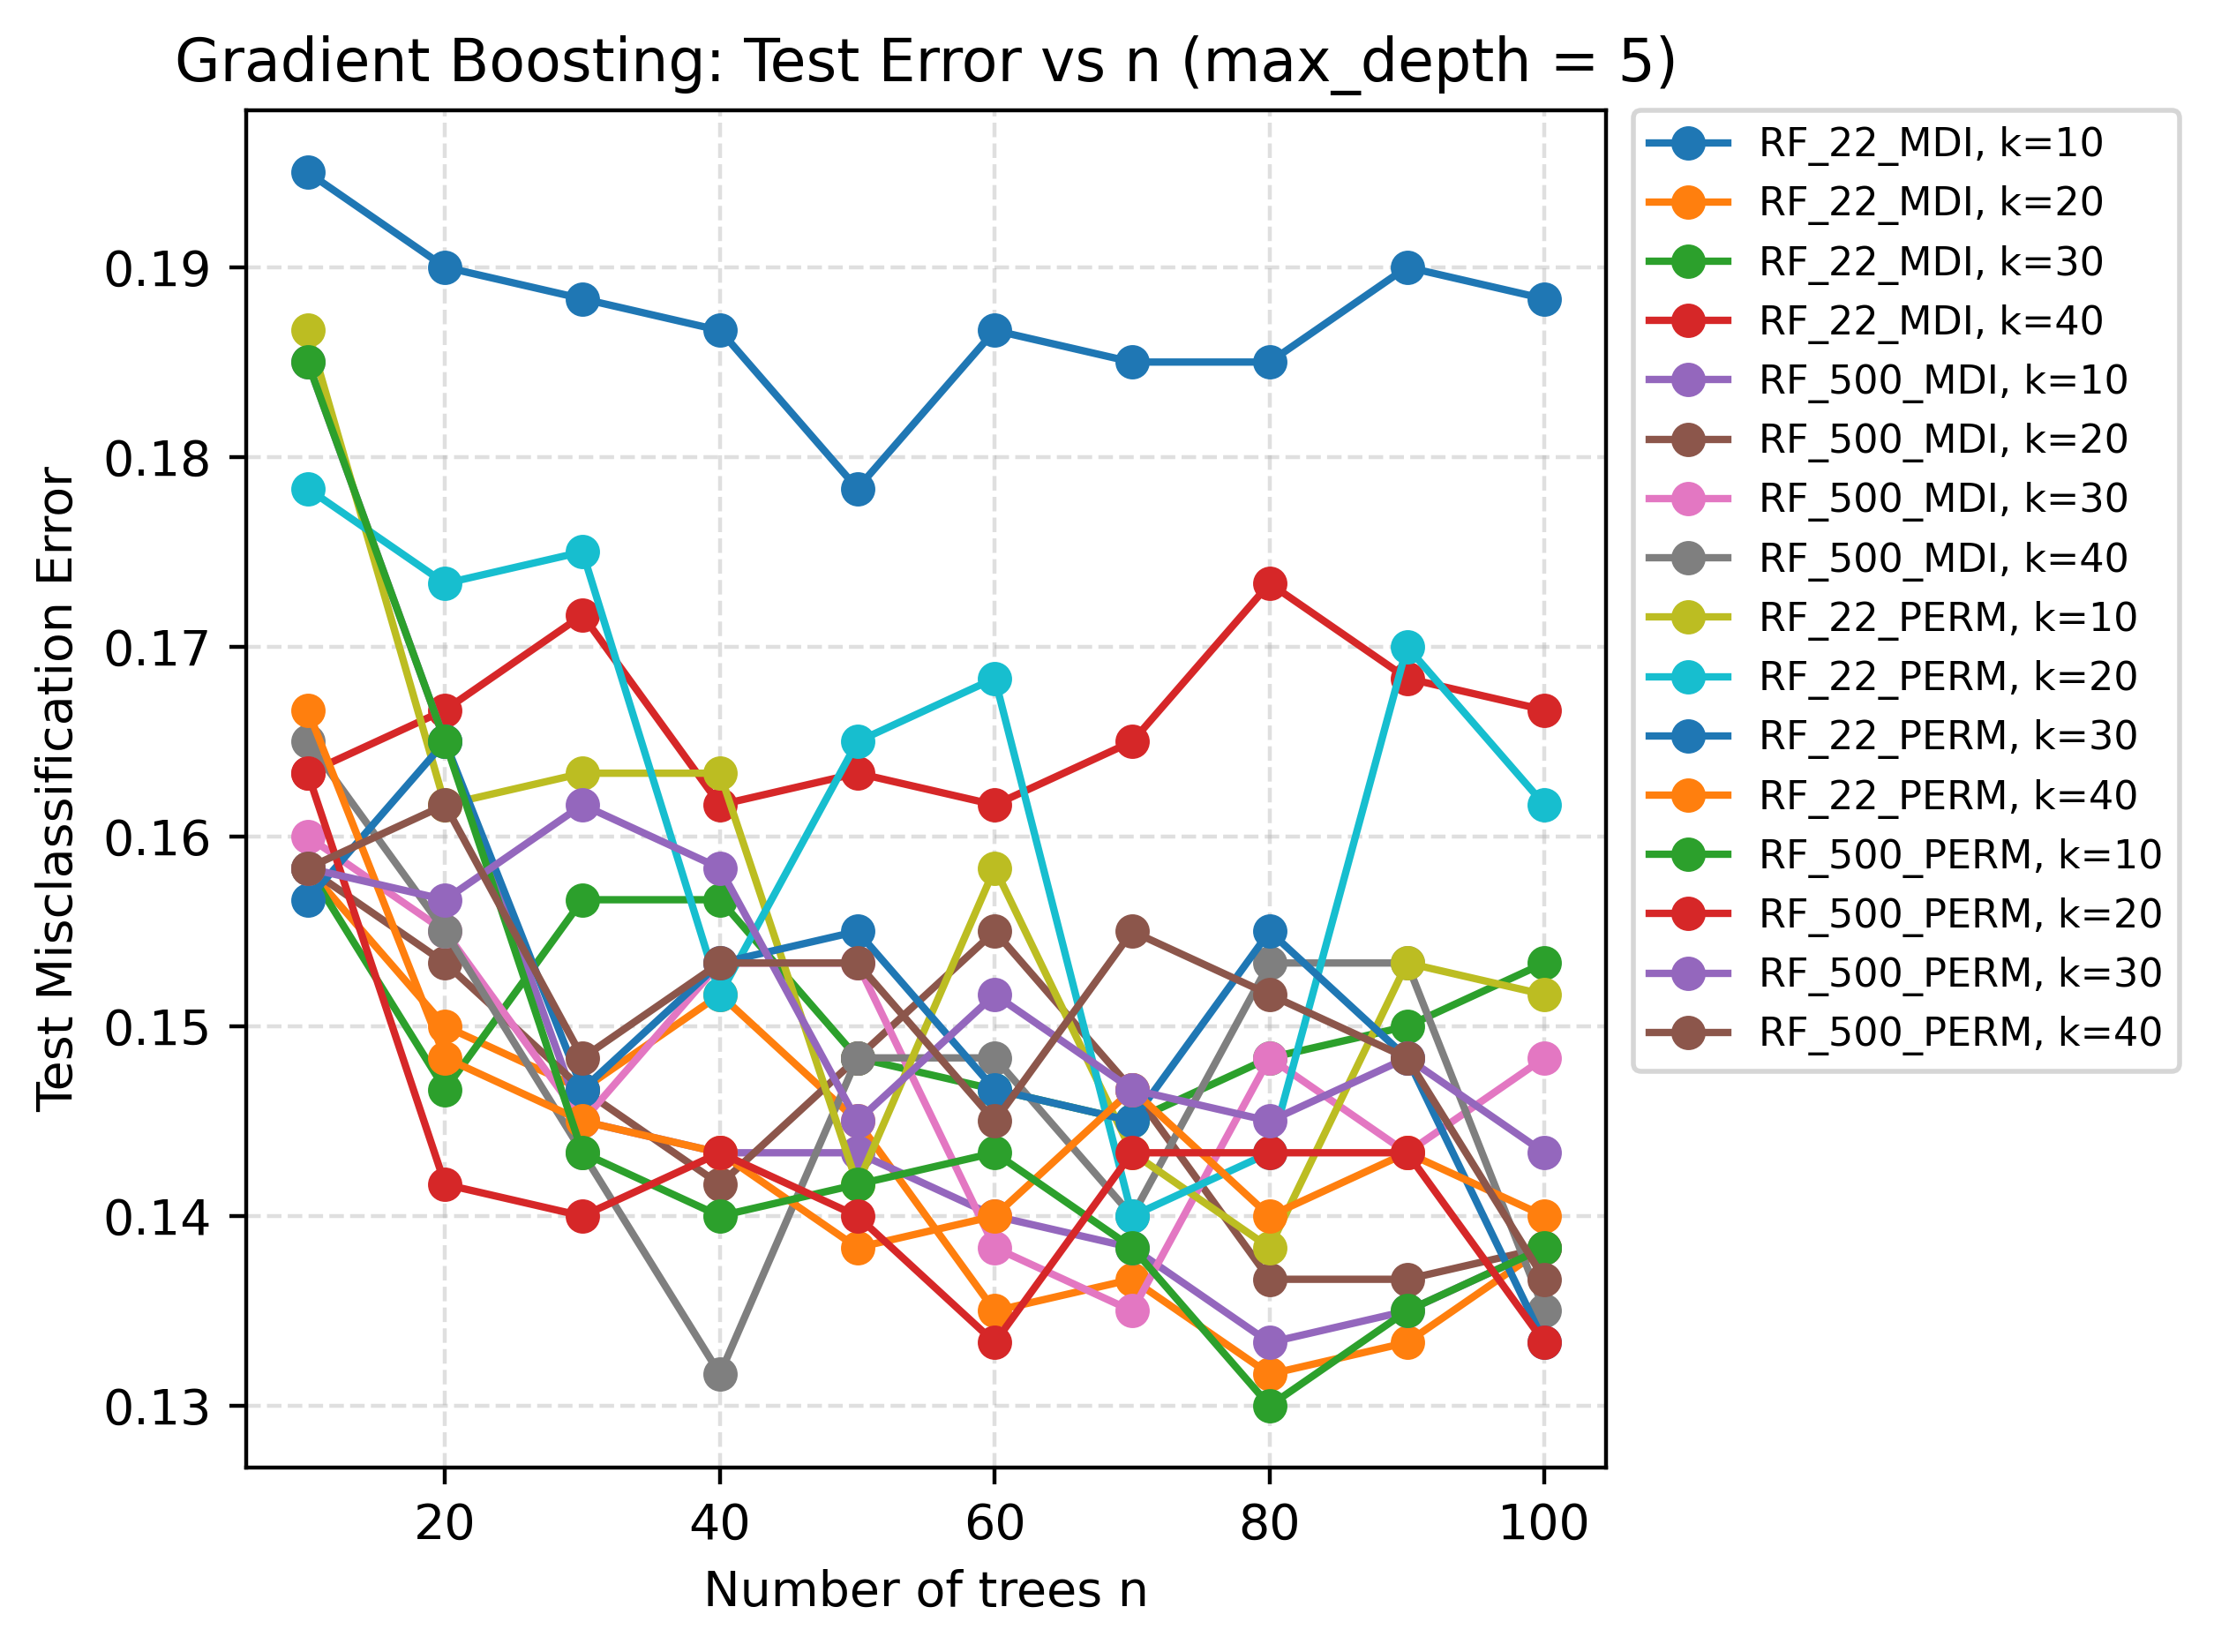
\includegraphics[width=0.7\linewidth]{../figures/gb_test_error_depth_5.png} 
        \caption{Test Errors vs. \(n\) for the 16 classifiers.  d=5} 
    \label{fig:test_error_d5} 
    \end{figure}
    Of the 320 classifiers, we can report the configuratio with the lowest test error in table: \ref{tab:table_part_d}
    \begin{table}[htbp]
        \centering
        \input{../output/smallest_test_error.tex}
        \caption{Configuration with smallest test error.}
        \label{tab:table_part_d}
    \end{table}
    \item Of the models, the random forest classifier from part c using selecting the 30 most importance
    as determined by MDI where each split is from all 500 features has the lowest test error of 0.11667.  
\end{enumerate}

\newpage
\newpage
%adding code
\appendix
\section*{Code}
%\lstinputlisting[language=Python]{../code/hw05.py}

\end{document}